\documentclass{bioinfo}
\copyrightyear{2021} \pubyear{2021}

%\access{Advance Access Publication Date: Day Month Year}
%\appnotes{Applications Note}

\begin{document}
%\firstpage{1}

\subtitle{GENOME ANALYSIS}

\title[StainedGlass]{StainedGlass: Making colorful dot-plots of genomic sequence}
\author[Vollger \textit{et~al}.]{
	Mitchell R. Vollger\,$^{\text{\sfb 1,}*}$,
	Peter Kerpedjiev\,$^{\text{\sfb 2}}$, 
	Adam M. Phillippy\,$^{\text{\sfb 3,*}}$, 
	and Evan E. Eichler\,$^{\text{\sfb 1,4,}*}$}
\address{
	$^{\text{\sf 1}}$Genome Sciences,
		University of Washington School of Medicine,
	 	Seattle, WA, USA \\
	$^{\text{\sf 2}}$Reservoir Genomics LLC,
	 Oakland, CA \\
	$^{\text{\sf 3}}$Genome Informatics Section,
		National Human Genome Research Institute, National Institutes of Health, Bethesda, MD, USA \\
	$^{\text{\sf 4}}$Howard Hughes Medical Institute, University of Washington, Seattle, WA, USA.
}

\corresp{$^\ast$To whom correspondence should be addressed.}

\history{}%Received on XXXXX; revised on XXXXX; accepted on XXXXX}
\editor{}%Associate Editor: XXXXXXX}

\abstract{
\textbf{Summary:} 
Visualization of genomic repeats is often accomplished through the use of 
dot plots; however, the emergence of telomere-to-telomere assemblies 
with multi-megabase repeats requires new visualization strategies. Here, 
we introduce StainedGlass which can generate publication quality figures 
that communicate the identity and orientation of 
multi-megabase repeats while scaling to entire genomes. \\
\textbf{Availability and implementation:} 
StainedGlass is implemented using \href{https://snakemake.github.io/}{snakemake}
and is available open source under the MIT license at 
\href{mrvollger.github.io/StainedGlass/}{mrvollger.github.io/StainedGlass/}.\\
\textbf{Contact:} \href{mvollger@uw.edu}{mvollger@uw.edu}\\
}

\maketitle

\section{Introduction}
Dot plots are a useful way to show sequence similarity... 

However, with increasingly contiguous assemblies of reference genomes (VGP) and complete human chromosomes (chr8, chrX, T2T) repeat structures including centromeres and other hererochromatic arrays are now for the first time available for analysis. The size and complexity of these structures, often many megabase pairs in humans, elude traditional dot plots for two reasons: 1) current visualization methods are largely based on perfect k-mer matches which do not lend themselves to the expected gaps and mismatches between large repeats, and 2) for tandem arrays of consisting of megabases of sequence dot plots are often just black squares that relay little information other the the size and presence of sequence similarity. 

In order to examine the centromere in human chr8 a colored dot plot based on sequence alignment rather than small k-mers was designed which allowed the authors to make a model for centomere evolution.  

In this work, we present StainedGlass, which generalizes the idea of colored dot plots based on sequence alignment and provides an easy, scale-able, and customize-able workflow so that it can be applied to new genomes. 

\section{Usage and examples}
\citealp{Boffelli03} example cite
\\
The tool is made available using snakemake which allows for reproducible and scalable data analyses.
Additionally, stability of new changes is automatically tested with each new change with continuous integration via github actions.

% \begin{itemize}
% \item for bulleted list, use itemize
% \item for bulleted list, use itemize
% \item for bulleted list, use itemize\vspace*{1pt}
% \end{itemize}

% \begin{table}[!t]
% \processtable{This is table caption\label{Tab:01}} {\begin{tabular}{@{}llll@{}}\toprule head1 &
% head2 & head3 & head4\\\midrule
% row1 & row1 & row1 & row1\\
% row2 & row2 & row2 & row2\\
% row3 & row3 & row3 & row3\\
% row4 & row4 & row4 & row4\\\botrule
% \end{tabular}}{This is a footnote}
% \end{table}


%%%%%%%%%%%%%%%%%%%%%%%%%%%%%%%%%%%%%%%%%%%%%%%%%%%%%%%%%%%%%%%%%%%%%%%%%%%%%%%%%%%%%
%
%     please remove the " % " symbol from \centerline{\includegraphics{fig01.eps}}
%     as it may ignore the figures.
%
%%%%%%%%%%%%%%%%%%%%%%%%%%%%%%%%%%%%%%%%%%%%%%%%%%%%%%%%%%%%%%%%%%%%%%%%%%%%%%%%%%%%%%

\begin{figure}[!tpb]%figure1
\centerline{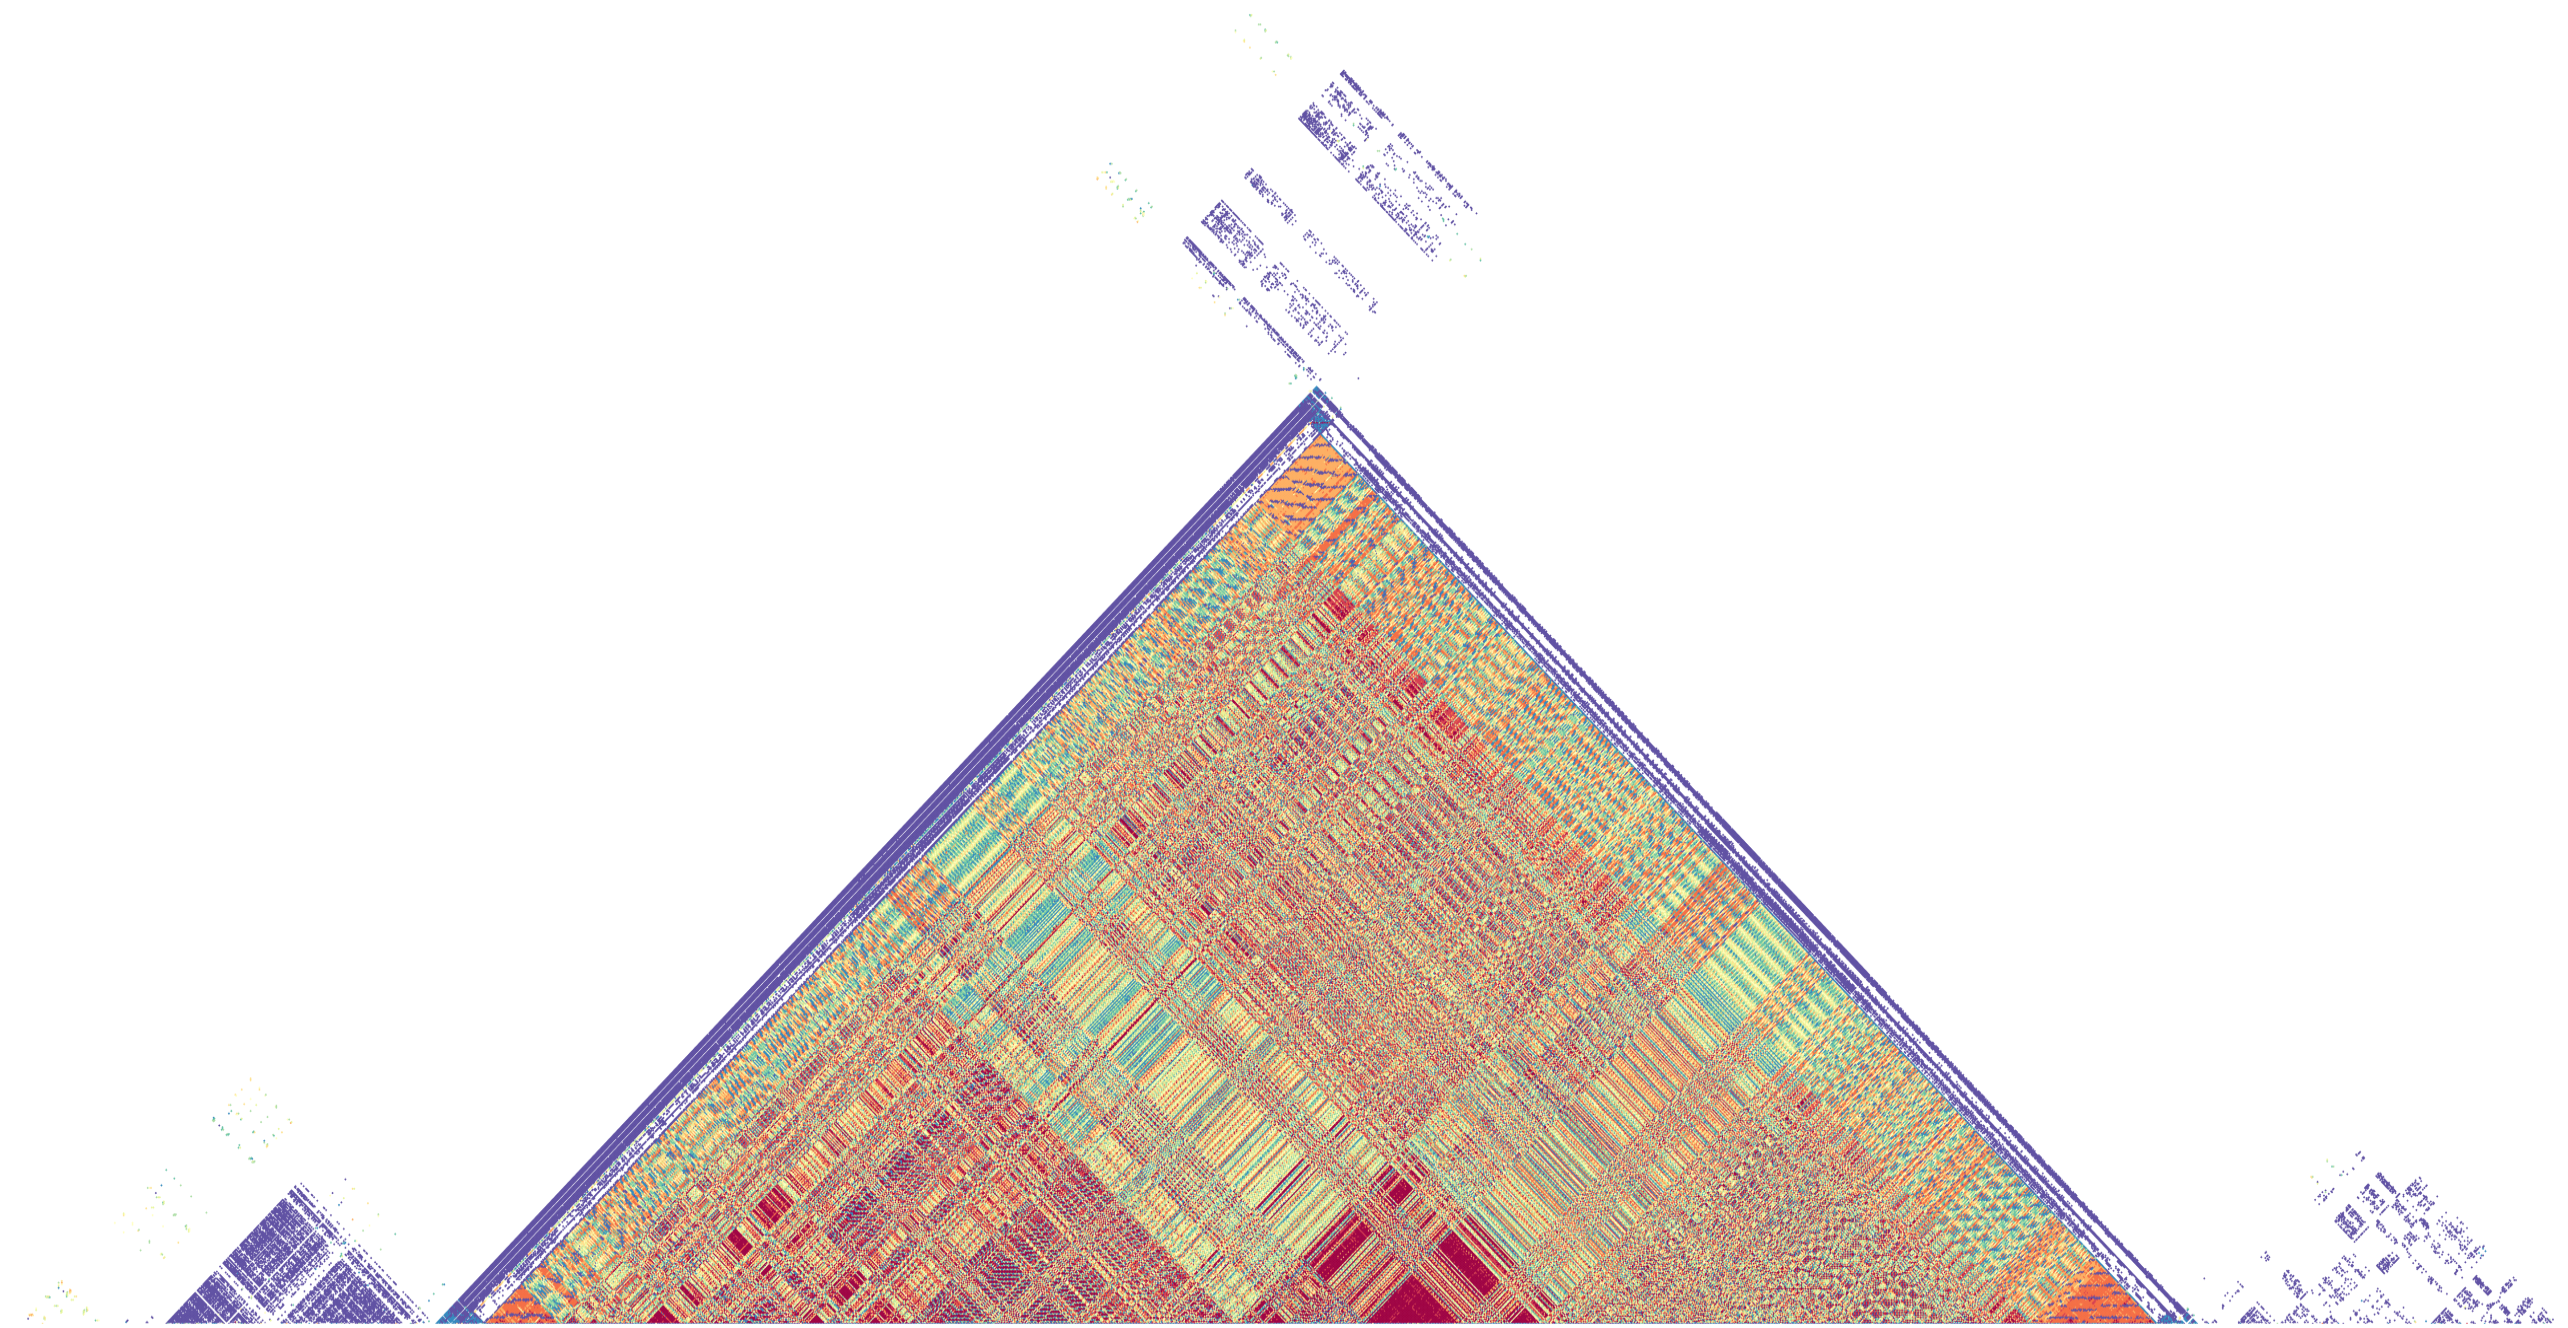
\includegraphics[width=0.5\textwidth,keepaspectratio]{../images/chr8.png}}
\caption{Caption, caption.}\label{fig:01}
\end{figure}
Figure~\ref{fig:01} 


\section{Conclusion}
Rust-Bio is a general purpose bioinformatics library. Building on the innovative Rust programming language, Rust-Bio combines memory safety with speed, complemented by rigorous continuous integration tests. So far, a wide set of algorithms and data structures for biological sequences is provided, ranging from index data structures to pattern matching and alignment, complemented by readers and writers for common file formats.

\section*{Acknowledgements}
The authors thank T. Brown for help in editing this manuscript 
and G. A. Logsdon for aesthetic suggestions.

\section*{Funding}
This work was supported, in part,
by the Intramural Research Program of the National Human Genome Research Institute,
National Institutes of Health (A.M.P.) and grants from the U.S. National Institutes of
Health (NIH grants 5R01HG002385 to E.E.E.; 5U01HG010971 to E.E.E.; and 1U01HG010973 to
E.E.E.). E.E.E. is an investigator of the Howard Hughes Medical Institute.

%\bibliographystyle{natbib}
%\bibliographystyle{achemnat}
%\bibliographystyle{plainnat}
%\bibliographystyle{abbrv}
%\bibliographystyle{bioinformatics}
%
%\bibliographystyle{plain}
%
%\bibliography{Document}


\begin{thebibliography}{}

\bibitem[Bofelli {\it et~al}., 2000]{Boffelli03}
Bofelli,F., Name2, Name3 (2003) Article title, {\it Journal Name}, {\bf 199}, 133-154.


\end{thebibliography}
\end{document}
